\section{Methods}
Our method models two types of signal from the data: (i) imbalance of the allele distributions at SNP loci (discussed in Section \ref{ss:allele_distrib}), and (ii) number of fragments sequenced from \ntilde1kb genomic regions (discussed in Section \ref{ss:coverage}). Though each of these is noisy, the two are (nearly) independent (modulo number of reads overlapping the SNP position) variables and can be combined into a single generative model. For this purpose we use a Hidden Markov Model (HMM), where we interpret the allele counts at SNP loci as emissions, while the coverage is used as a prior probability for each state (see Section \ref{ss:hmm}). 

For our method we assume that we have phased haplotypes of both parents, and deep sequencing data of cfDNA from maternal plasma. In practice we used whole genome sequencing (WGS) data for the parents, with phasing based on 1000 Genomes data (see Section \ref{data}). All \textit{de novo} CNVs thus correspond to a particular parental haplotype duplication or deletion event. Labelling the two maternal and paternal haplotypes as $M_A,M_B,P_A,P_B$. For each inheritance pattern -- normal inheritance, maternal duplication, paternal duplication, maternal deletion, paternal deletion -- we introduce a set of \textit{phased inheritance patterns} that enumerates all the possible configurations of fetal haplotypes corresponding to the respective inheritance pattern. For example a duplication in the maternal gamete will consist of one (or more) of six phased inheritance patterns:
\begin{align*}
M_AM_AP_A, ~~M_AM_BP_A, ~~M_BM_BP_A,\\
M_AM_AP_B, ~~M_AM_BP_B, ~~M_BM_BP_B
\end{align*}
There are a total of 20 phased inheritance patterns ($\PP$): 6 each for maternal/paternal duplication, 2 each for maternal/paternal deletion, and 4 for normal inheritance). We refer to the number of alleles (copy count) inherited by the fetus as $|\PP|$. We use $r$ to refer to the percentage of cfDNA that is fetus-derived; this parameter is estimated from positions in the genome where the parents are homozygous for alternate alleles.

\subsection{SNP Allele Distribution}\label{ss:allele_distrib}
For every SNP locus we observe a distribution of nucleotides in maternal plasma reads. In this section we focus on calculating the probability of the observation with respect to a phased inheritance pattern. Formally, we observe the counts of the 4  nucleotides $\{k_\A, k_\C, k_\G, k_\T\}$ and compute the probability of observing each of these from a particular phased inheritance pattern $\PP$ based on the  Poisson distribution, approximated by a Gaussian, i.e.
\begin{align}
Pr[k_x ~|~  M_A, M_B; P_A, P_B; r; \PP] \sim \N\(\mu_x, \mu_x\)
\end{align}
To compute the expected support $\mu_x$ for $x\in\{\A,\C,\G,\T\}$, we first adjust the mixture ratio $r$  based on the expected number of fetal haplotypes $|\PP|$, as absence/presence of an additional fetal copy in the plasma sample influences the local fetal mixture ratio. We accommodate this influence of $|\PP|$ expected fetal haplotypes instead of regular two as follows:
\begin{align}
r' =&  \frac{ |\PP| \cdot r/2 }{|\PP| \cdot r/2 ~+~ (1-r) }
\end{align}
Then for each nucleotide $x$ we compute the probability $p_x$ of observing a read supporting $x$. Such a read might have originated from multiple haplotypes, including two maternal haplotypes and $|\PP|$ fetal haplotypes. We can individually evaluate this probability for each haplotype and subsequently sum them to obtain $p_x$:
\begin{align}
p_x &= \sum_{i \in \{A,B\} } [M_i \text{ equals } x] \cdot m_i (1-r') \\ %& \text{//maternal haplotypes with $x$ variant}\\
	&~~~ + \sum_{y \in \PP} [y \text{ equals } x] \cdot \frac{r'}{|\PP|} \nonumber % & \text{//fetal haplotypes with $x$ variant} \nonumber
\end{align}
For reads putatively coming from maternal portion of the cfDNA sample, we correct for maternal CNVs by using the allele ratios $m_i$ as observed in maternal-only sequencing data. Additionally, in order to mitigate noise we add pseudocount $\alpha$ (proportional to the genome-wide coverage) to these counts.
\begin{align}
m_i &= \frac{\alpha + \# \text{reads supporting }M_i\text{ in maternal sample}}{2\alpha + \sum_{j \in \{A,B\} }\# \text{reads supporting }M_j\text{ in maternal sample}}
\end{align}
We thus obtain the expected probability distribution for each nucleotide observed at this SNP locus.  To get the expected number of reads supporting particular variant at this SNP locus, we have to multiply $p_x$ by the number of reads mapped,
\begin{align}
\mu_x &= p_x \cdot \#\text{mapped reads}
\end{align}
As we describe later, we use this probability distribution $\N\(\mu_x, \mu_x \)$ that is conditional on phased pattern $\PP$ as the emission distribution for each nucleotide in our HMM.

\subsection{CNVs and Depth of Coverage}\label{ss:coverage}
\begin{figure}
\caption{Distribution of fragments per kilobase of chromosome 1 per million fragments (FPKM) in 1 megabase segments for plasma sample (blue) and maternal sample (red) of the I1 trio.}
\label{fig:fpkm}
\centering
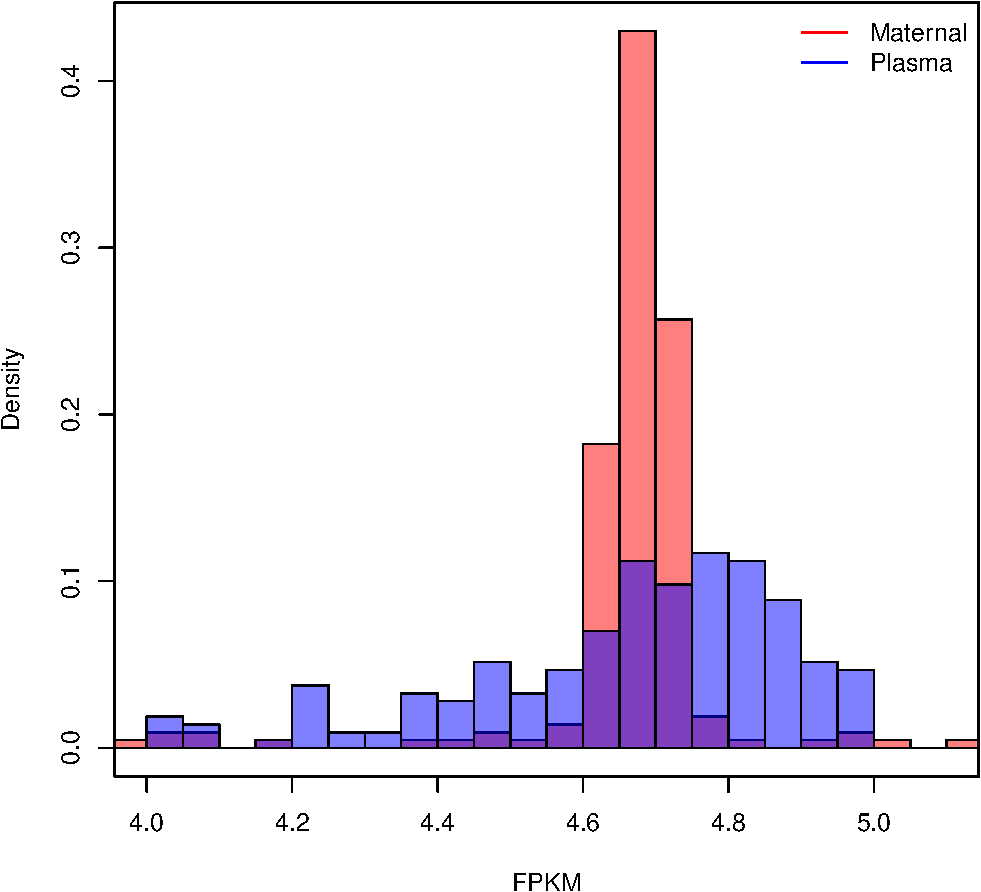
\includegraphics[height=0.33\textheight]{figures/histo-crop}
\end{figure}

\begin{figure*}
\caption{(a) A scatterplot demonstrating the correlation of window ratio values (WRV) between plasma samples of I1 and G1 trios. The shown WRVs were computed for windows of size 1kb in chromosome 1. (b) Histogram of absolute errors between WRVs from different samples; comparing distribution of absolute error between plasma samples of I1 and G1 trios (red), and between plasma sample and maternal sample of I1 trio (blue). There is a notably heavier tail in case of plasma to maternal sample error distribution, composed of windows with weak WRV correspondence -- an artifact of wider coverage distribution in plasma cfDNA sample compared to standard WGS maternal sample (Figure \ref{fig:fpkm}). This artifact causes plasma to maternal sample WRV comparison to have higher mean absolute error (0.000521, compared to 0.000347 for plasma I1 to plasma G1) even though they are from the same trio. }
\label{fig:wrv}
%\missingfigure{The main HMM}
\subfigure[]{ %\label{fig:scatter:a}
\begin{minipage}[b]{0.48\textwidth}
	\centering
	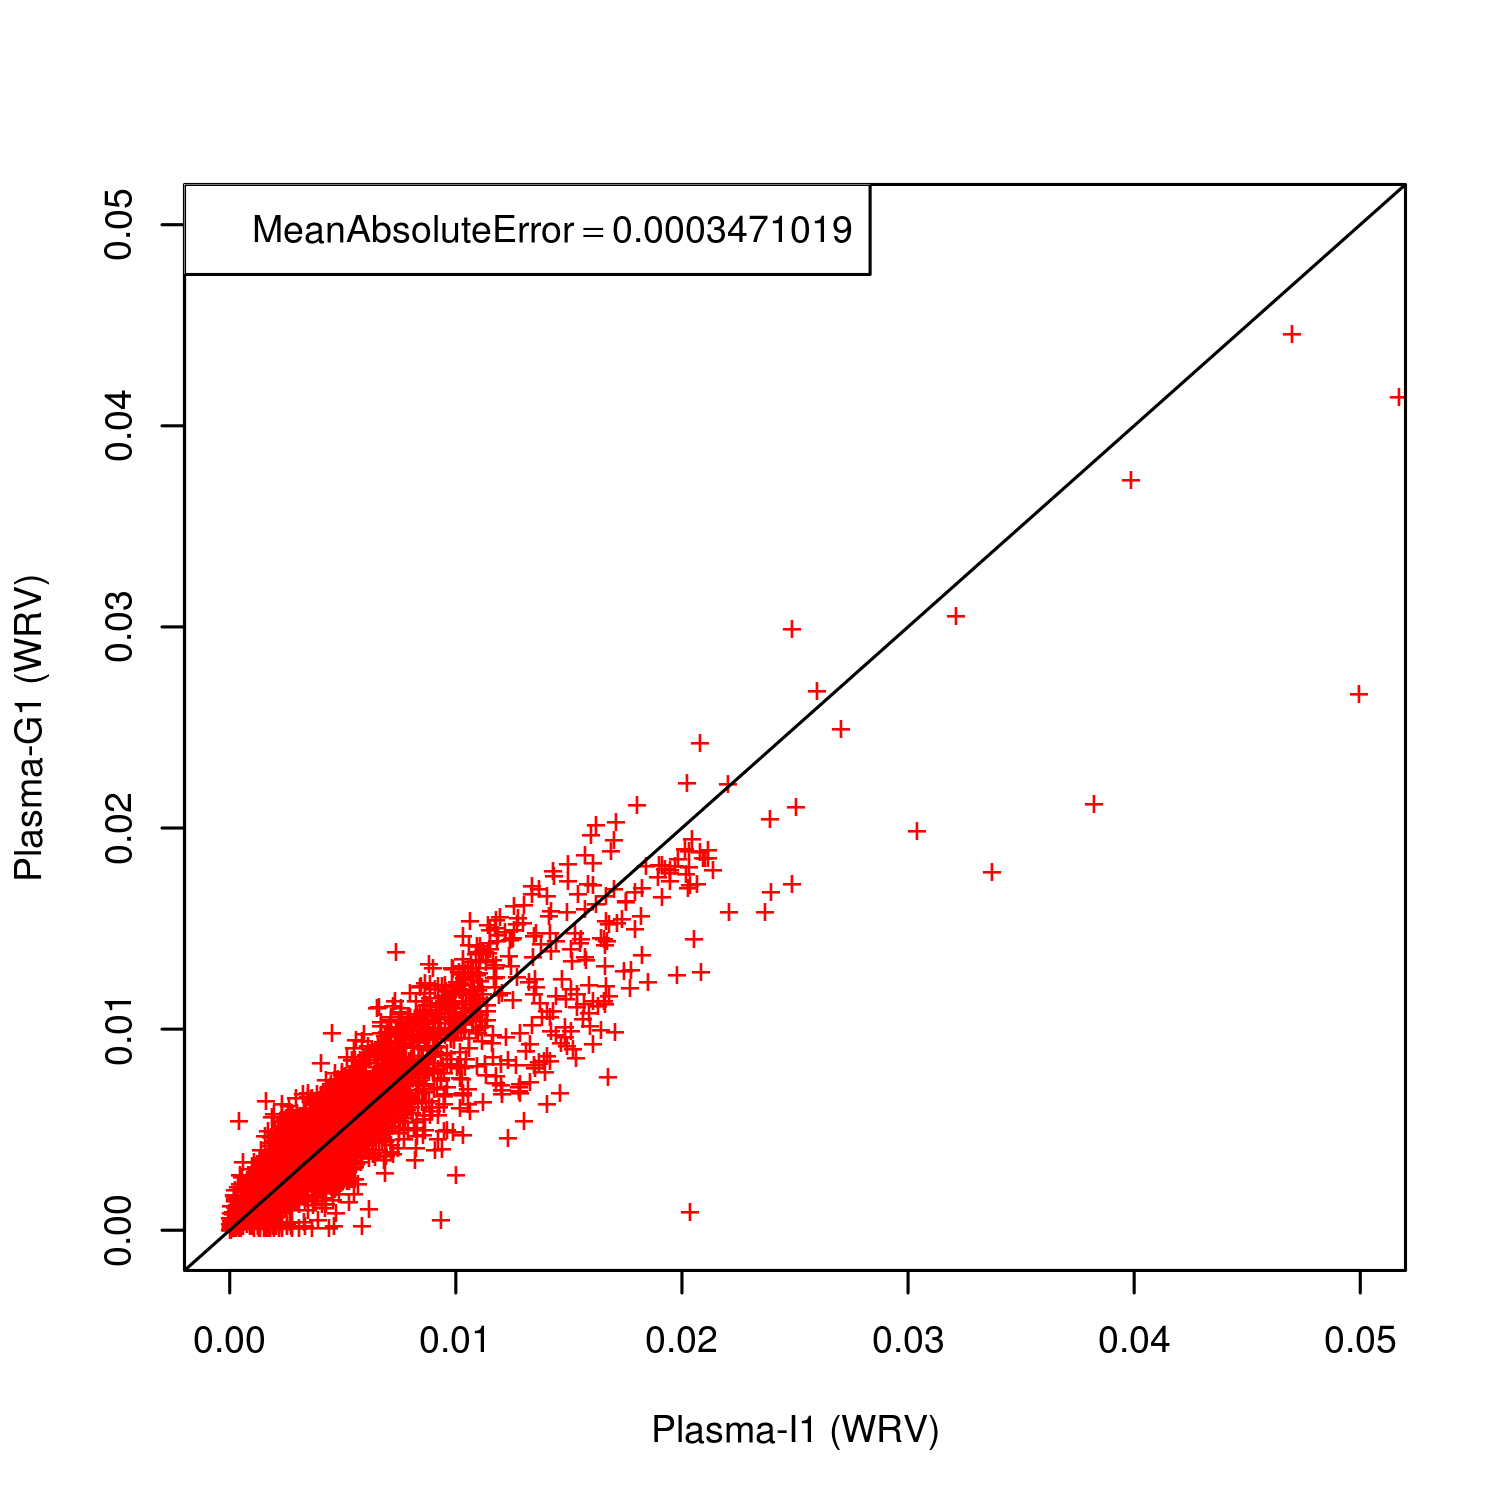
\includegraphics[width=0.98\textwidth]{figures/IpGp}
	\end{minipage}	
}
\hspace*{10pt}
\subfigure[]{ %\label{fig:histo:b}
	\begin{minipage}[b]{0.48\textwidth}
		\centering
	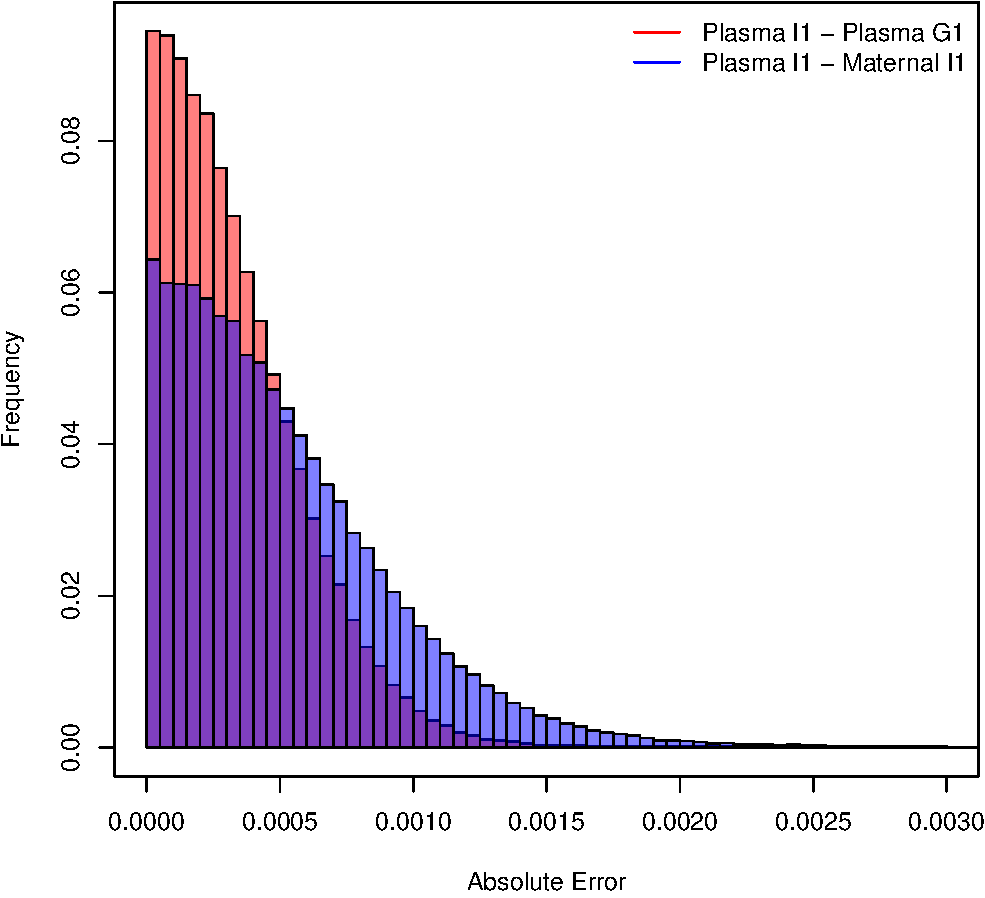
\includegraphics[width=0.98\textwidth]{figures/wrv_error_histo}
	\end{minipage}	
}
\end{figure*}

Variations in number of fragments sequenced per a region is a standard measure used for detection of mid to large sized CNVs (see \cite{medvedev2009} for a review), and has also been used for CNV detection from maternal plasma \citep{srinivasan2013, chen2013}. However the relatively low admixture of fetal DNA in the maternal plasma together with cfDNA sequencing biases considerably limit potential of methods relying on coverage signal from a single sample. Furthermore, the high variability of the coverage derived from blood plasma (Figure \ref{fig:fpkm}) makes it difficult to identify shorter CNVs. Thus methods \cite{srinivasan2013, chen2013} use large bins and require multiple datasets to establish a baseline for CNV calling.

Simultaneously, the coverage forms an important complementary signal to the allelic distributions described above: certain ratios have very similar probability under different phased patterns, e.g. a deletion of a maternally inherited allele may yield distributions similar to a paternally inherited duplication. Incorporating the coverage signal helps to discriminate such states. In our method, we use the coverage information as a noisy predictor to complement the signal we obtain from SNP loci.

As a measure of coverage in a genomic region we use \emph{window ratio value} (WRV) analogous to the \emph{bin ratio value} measure used by \cite{srinivasan2013}, which is essentially the number of fragments mapped to the region and normalized by the number of fragments mapped to other regions with similar $\G\C$ content. Note that window ratio values are independent of $\G\C$ content and depth of sequencing of the sample.

For the purpose of our model, we split the genome to non-overlapping windows, each containing a single SNP, with breakpoints being in the middle between two adjacent SNPs. For each SNP $i$ the corresponding $\WRV_i$ for the window $W_i$ containing the $i$-th SNP position is then computed as the ratio of number of fragments $N_{W_i}$ mapped to $W_i$ to the sum of fragments mapped to 200 windows of the same size with $\G\C$ content closest to $W_i$:
\begin{align}
\WRV_i &= \frac{ N_{W_i} }{ \mathlarger{\sum_{W \in neigh_{\G\C}^{200}(W_i)}} N_{W} }
\end{align}
However, the variable length of the windows makes such computations expensive as computation of $neigh_{\G\C}^{200}(W_i)$ is linear in number of windows. To make the WRV computations practical, we scale $N_{W_i}$ to correspond to expected number of fragments as if $|W_i| = 1$kb by multiplying $N_{W_i}$ by $1000/|W_i|$ (for clarity, not shown in our equations). Then WRVs in 1kb bins can be precomputed, enabling us to find $neigh_{\G\C}^{200}(W_i)$ in time logarithmic from the number of bins.
Using 1kb bins is a good approximation as the mean distance between two adjacent SNP loci is expected to be 1kb.

Overall, our goal is to estimate the probability of observing $\WRV_i^S$ in the studied plasma sample conditional on the number of fetal haplotypes ($|\PP|$), which is either three for duplication, one for deletion, or two for normal inheritance. To do so, we use a reference sample to obtain $\WRV_i^R$ for comparison (computed in the same genomic window $W_i$). Further we need to compute two more reference $\WRV_i^R$s, each scaled to reflect one CNV type. For duplication, we would expect to see $(1+r/2)$ times more fragments while for deletion $(1-r/2)$ times less fragments, thus the scaled $\WRV_i^{R,|\PP|}$ is estimated as
\begin{align}
\WRV_i^{R,|\PP|} = \frac{ N_{W_i^R} \cdot \big(1+\(|\PP|-2\)\cdot r/2\big) }{ \mathlarger{\sum_{W \in neigh_{\G\C}^{200}(W_i^R)}} N_{W^R} }
\end{align}

Finally, we can compute the probability of $\WRV_i^S$ being generated from an event with fetal allele copy count $|\PP|$ as:
\begin{align}
\N(\WRV_i^{R,|\PP|}-\WRV_i^S; \mu=0, \sigma_{\text{noise}})
\label{eq:wrv_distrib}
\end{align}
where we model the difference between $\WRV_i^S$ and $\WRV_i^R$ as a Gaussian noise with zero mean and empirically estimated variance $\sigma_{\text{noise}}$.

By normalizing the probabilities of $\WRV_i^S$ w.r.t. all phased patterns, we obtain priors for each phased pattern that are used in the HMM described in the next section. 

As a reference plasma sequencing coverage we use plasma sample of the G1 trio of \cite{kitzman2012} dataset, as the overall coverages observed in corresponding bins between the two samples correlate well (mean absolute error of WRVs being 0.000347, see Figure \ref{fig:wrv}A). Since coverage variation of cfDNA from plasma has much wider distribution than standard WGS, a sample from other plasma is more suitable than the same trio maternal sample (see Figure \ref{fig:wrv}B) for purpose of coverage distribution reference in our model. Availability of additional plasma datasets would enable us to further improve the accuracy of the reference bins.

Note that compared to previous methods we use significantly smaller windows: \ntilde1kb versus 100kb-1Mb used previously by \cite{chen2013, srinivasan2013}. As mentioned earlier, our goal here is not to detect CNVs immediately, but to rather compute a probability distribution over the number of haplotypes the fetus has inherited, which are used as  priors in the more complex model. Due to the independence assumptions inherent in the HMM we want these priors, applied at each state, to be (approximately) independent, and hence we picked non-overlapping windows each containing one SNP locus.

\subsection{Hidden Markov Model for CNV Inference}\label{ss:hmm}
To combine the signals from individual SNP positions, we use an HMM with 20 states corresponding to modelled phased inheritance patterns (Figure \ref{fig:hmm_main}). That means each sate represents a possible set of parental haplotypes inherited by the fetus. States representing normal inheritance are central to the model assuming that two CNVs cannot be immediately subsequent. Between states of the same inheritance pattern, we allow for transitions reflecting either recombinations or errors in phasing. For each state, the emissions are the counts of individual alleles in reads mapped to that particular SNP position. The probability of the observed emission is the probability of such allele counts in the expected allele distribution conditional on phased inheritance pattern as described above in Section \ref{ss:allele_distrib}.

To incorporate the coverage information, for each SNP position we multiply the transition probabilities into the state by the copy number priors obtained in Section \ref{ss:coverage}. Specifically, each edge incoming to a state is multiplied by the corresponding prior of inheriting that many haplotypes, which are then normalized so that the sum of the probabilities leaving each state is one. %the transition probabilities  \ref{fig:hmm_main:a}

The transition probabilities within an event type (e.g. maternal duplication) were set to $0.01$, to reflect expected haplotype block lengths of several hundred SNPs. Further, the transition probability for starting a CNV was set to one in ten thousand SNP loci ($0.0001$) with length expected to span approximately one thousand SNPs (i.e. transition probability back to normal inheritance was set to $0.001$).

\begin{figure*}[t]
\caption{Hidden Markov model used for CNV inference. (a) High-level architecture of the HMM with 5 sets of states corresponding to 5 types of fetal inheritance. Note, we do not allow two CNVs to be adjacent, thus switching between two CNVs always has to go through a normal inheritance state. Edges in (a) represent edges coming in/out of all states between two sets of states. (b-d) Correspond to the diagram of states of the HMM within the normal inheritance, maternal duplication, and maternal deletion states of (a). Paternal duplications/deletions are analogous to (c) and (d). Inner edges in (b-d) serve to model errors in phasing or recombination events.}
\label{fig:hmm_main}
%\missingfigure{The main HMM}
\centering
\subfigure[Overall HMM architecture]{\label{fig:hmm_main:a}
	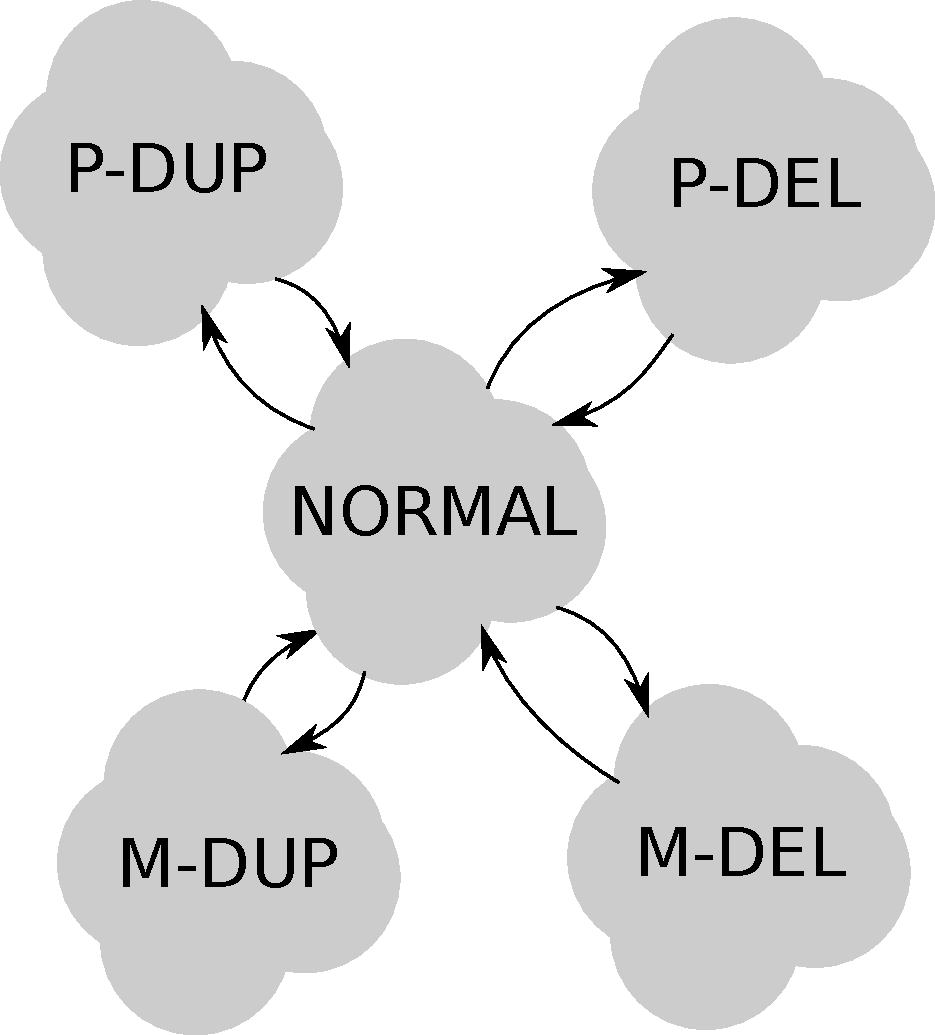
\includegraphics[height=0.2\textheight]{figures/main-HMM}
	\quad
}
\hspace{20pt}
\subfigure[States for normal inheritance]{
	\begin{minipage}[b]{0.45\textwidth}
		\centering
		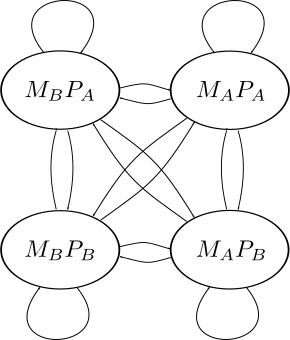
\includegraphics[height=0.2\textheight]{figures/NOR-HMM}
		\vspace{8pt}
	\end{minipage}	
}

\vspace{10pt}
\subfigure[States for maternal duplication]{
\begin{minipage}[b]{0.4\textwidth}
	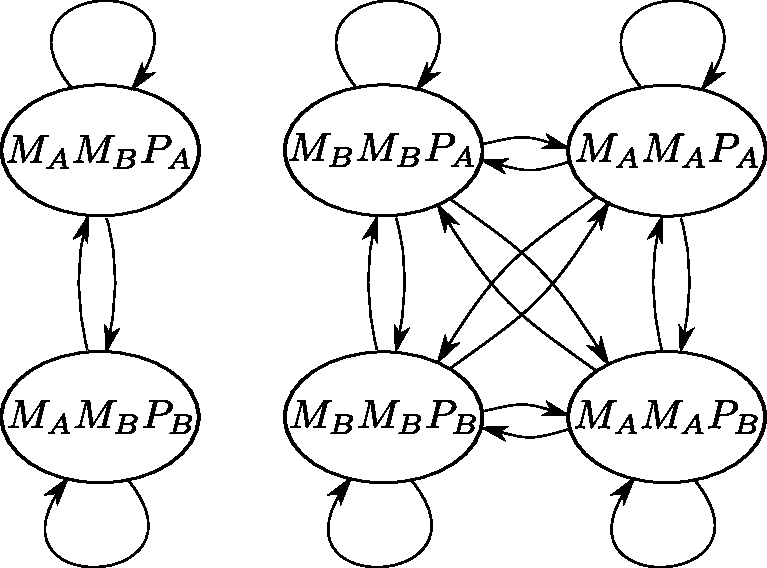
\includegraphics[height=0.2\textheight]{figures/DUP-HMM}
	\end{minipage}	
}
\hspace{0pt}
\subfigure[States for maternal deletion]{
	\begin{minipage}[b]{0.4\textwidth}
		\centering
		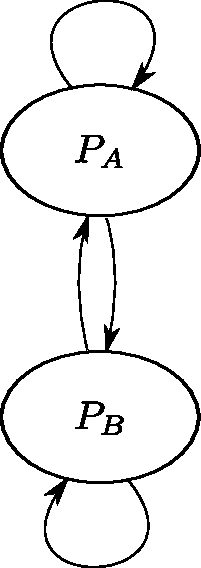
\includegraphics[height=0.2\textheight]{figures/DEL-HMM}
	\end{minipage}	
}
\end{figure*}

\input simulation
